
\chapter{Grundlagen der Programmierung}
\label{c:grundlagen}
\setcounter{page}{1}
\subsubsection{Was ist Progrmamieren?}

Schauen wir zunächsteinmal, was einige der „großen Köpfe“ der
Informatik das Programmieren definieren.

\begin{quote}
	"To program is to understand" \\
	\textit{~ Kristen Nygaard}
\end{quote}

\begin{quote}
	„Programming is a Good Medium for Expressing Poorly
	Understood and Sloppily Formulated Ideas“\\
	\textit{~ Marvin Minsky, Gerald J. Sussman}
\end{quote}

\subsubsection{Strukturierungsmechanismen einer
Programmiersprache}

Eine Programmiersprache ist mehr als ein Hilfsmittel um einen
Computer anzuweisen, Aufgaben durchzuführen.
Sie dient auch als \textbf{Rahmen}, innerhalb dessen wir \textbf{unsere
Ideen} über die \textbf{Problemdomäne organisieren.}

Wenn wir eine Sprache beschreiben, sollten wir
die Hilfsmittel beachten, die sie uns zum
Kombinieren von einfachen Ideen anbietet, um
komplexere Ideen zu bilden.

Jede vollwertige Programmiersprache hat drei Mechanismen,
um Prozessideen zu strukturieren:

\begin{itemize}
	\item \textbf{\textit{Primitive} Ausrücke}
		\subitem - Repräsentieren die einfachsten Einheiten der Sprache
		\subitem - Im Deutschen: jedes Wort ist ein primitiver Ausdruck
	\item \textbf{\textit{Kombinationsmittel}}
		\subitem - Zusammengesetzte Elemente werden aus einfacheren Einheiten
		konstruiert
		\subitem - Im Deutschen: Zusammensetzung mehrerer Wörter zu einem Satz.
	\item \textbf{\textit{Abstraktionsmittel}}
		\subitem - Zusammengesetzte Elemente können benannt und weiter als Einheiten manipuliert werden
		\subitem - Im Deutschen: Definition eines Begriffs („Ein Auto ist ...“), so dass der Begriff danach als „Kurzform“ für die Erklärung nutzbar ist
\end{itemize}

\section{Strukturierungsmechanismen}
\subsection{in der Elektronik:}
\begin{itemize}
	\item \textbf{\textit{Primitive} Ausrücke}
		\subitem - Widerstände, Kondensatoren, Induktivitäten, Spannungsquellen, ...

	\item \textbf{\textit{Kombinationsmittel}}
		\subitem - Richtlinien für das Verdrahten der Schaltkreise
		\subitem - Standardschnittstellen (z.B. Spannungen, Strömungen) zwischen den
		Elementen. Diese Schnittstellen können auch Anforderungen an
		konkrete zulässige Werte oder Einheiten stellen („5 mA“)

	\item \textbf{\textit{Abstraktionsmittel}}
		\subitem - 	“Black box” Abstraktion – denke über einen Unter-Schaltkreis als eine
		Einheit: z.B. Verstärker, Regler, Empfänger, Sender, ...
\end{itemize}


\section{Sprachelemente}

\subsection{Die Primitiven}
\subsubsection{Zahlen}
Zahlen sind selbstauswertend: Die Werte der Zifferfolge ist die Zahl,
die, die sie bezeichnen.
$$ 23 \Rightarrow 23 $$
$$ -36 \Rightarrow -36 $$

\subsubsection{Boolesche Werte}
Boolsche Werte können nur \textit{wahr} oder \textit{falsch} sein. Diese sind ebenfalls
selbstauswertend. Sie werden als $$True  oder  False$$ bezeichnet. 
Prozeduren sind in der Programmierung auch als "Funktionen" oder Methoden bekannt. Beispiele sind hierfür sind
$$ +, *, /, -, =, usw.$$
Aber was ist der Wert von so einem Ausdruck? Der Wert von + ist eine Prozedur, die Zahlen addiert. Dies werden wir später als "Higher-Order Procedures" kennen lernen.
% Was auch immer das folgende beeutet. steht aber so in den Folien :)
Auswertung: Nachschlagen des dem Namen zugewiesenen Wertes.

\subsection{Besonderheiten bei Zahlen}
DrRacket rechnet immer genau, wenn das möglich ist. Ganze und endliche Zahlen berechnet er wie so wie es "üblich ist". Brüche mit periodischem Ergebnis werden ebenfalls in einem Text als Bruch - etwa \fbox{\textit{7/3}} dargestellt. Im Programm werden sie jedoch als Periode angezeigt. Beispielsweise \fbox{- 2.\uline{3}}.
Doch können nicht jede Zahlen \textit{exakt} dargestellt werden. Man wird hier durch die verwendung des Binärsystems eingeschränkt. Es gilt:
\begin{quote}
	"je mehr Nachkommastellen die Zahl besitzt, desto ungenauer wird in der Regel ihre Darstellung im Binärsystem"
\end{quote}

Zahlen unendlicher Länge ohne Periode werden wie folgt dargestellt: \fbox{\#i \"'inexact\"'}\\
Hier einige Beispiele:
$$e: \fbox{\#i2.718281828459045}$$
$$pi: \fbox{\#i3.141592653589793}$$
$$\sqrt{2}: \fbox{\#1.4142135623730951}$$

Mit Brüchen oder „inexakten“ Zahlen kann normal gerechnet
werden – das Ergebnis ist aber ggf. wieder „inexact“
$$(\sqrt{2})^2 = \fbox{\#i2.0000000000000004}$$

\subsection{Kombination}
Der Wert einer Kombination wird bestimmt durch die Ausführung der (durch den Operator) angegebenen Prozedur mit den Werten der Operanden. In Racket ist eine Sequenz von Ausdrücken eingeschlossen in Klammern. Die Ausdrücke sind primitiv oder erneut zusammengesetzt.



Hier ein Beispiel:
Numerische Ausdrücke können mit Ausdrücken kombiniert werden,
die primitive Prozeduren repräsentieren (z.B. + oder *), um einen
zusammengesetzten Ausdruck zu erstellen.
Kombinationen können verschachtelt werden. Dafür müssen sie die Regeln einfach Rekursiv anwenden.
\begin{figure}
	\begin{center}
		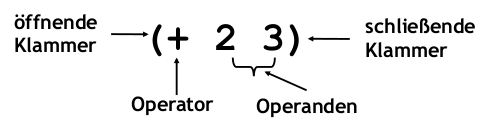
\includegraphics[height=2cm]{Bilder/T01_Sprachelemente_Kombination}
		\caption{}\label{t01_sk}
	\end{center}
\end{figure}

\begin{lstlisting}{t01_prog1}
(+ 4 (* 2 3)) = (4 + (2 * 3)) = 10
(* (+ 3 4) (- 8 2))
= ((3 + 4) * (8 - 2))
= 42
\end{lstlisting}

WICHTIG:
 Eine Kombination bedeutet immer eine Anwendung einer Prozedur. Klammern können nicht eingefügt oder weggelassen werden, ohne die Bedeutung des Ausdrucks zu ändern.

\subsection{Abstraktion}
